\documentclass[12pt]{extarticle}
\usepackage[utf8]{inputenc}
\usepackage{cite}
\usepackage{listings}
\usepackage{color}
\usepackage{graphicx}
\usepackage{amsmath}

\definecolor{dkgreen}{rgb}{0,0.6,0}
\definecolor{gray}{rgb}{0.5,0.5,0.5}
\definecolor{mauve}{rgb}{0.58,0,0.82}

\lstset{frame=tb,
  language=Python,
  aboveskip=3mm,
  belowskip=3mm,
  showstringspaces=false,
  columns=flexible,
  basicstyle={\small\ttfamily},
  numbers=none,
  numberstyle=\tiny\color{gray},
  keywordstyle=\color{blue},
  commentstyle=\color{dkgreen},
  stringstyle=\color{mauve},
  breaklines=true,
  breakatwhitespace=true,
  tabsize=3
}

\title{Implementing PPO in Pytorch}
\author{Abhijeet Ghawade}
\date{March 2019}

\begin{document}

\maketitle
\section{Introduction}
This is a detailed explaination for implementing PPO (Proximal Policy Optimization ) paper, we will go through the maths and the code simultaneously to understand what is the general method to implement papers in Deep-RL specifically. \\
I have used PyTorch for implementing the Neural Network. \\
This is hardcoded for atari gym environments, but with a few changes, you can use it for any other environment required. 
I will follow a causal approach for the code, I hope which will be best for understanding the implementation best.We will understand the intuition for the paper as we go along. \\


We will run the code as the Main program, or else, it can be used as a Module to be imported. 
\begin{lstlisting}
if __name__ == "__main__":
	m=Main()
	m.run_training_loop()
	
	m.record_video()
	m.destroy()
\end{lstlisting}

\section{class Main()}
We first run the class Main, beginning with it's initializations, 

\begin{lstlisting}
class Main(object):
	def __init__(self):

		self.gamma=0.99
		self.lamda=0.95
		self.updates=15000
		self.epochs= 4 
		self.n_workers= 8
		self.worker_steps=128
		self.n_mini_batch=4
		self.batch_size=self.n_workers*self.worker_steps  #[8*128=1024]
		self.mini_batch_size=self.batch_size // self.n_mini_batch  #[1024/4=256]
		np.random.seed(1)
		torch.manual_seed(1)


		assert(self.batch_size%self.n_mini_batch==0)
		random_worker_seed=12
		self.workers=[Worker(random_worker_seed+i) for i in range(self.n_workers)]
		self.obs= np.zeros((self.n_workers,84,84,4),dtype=np.uint8)

		for worker in self.workers:
			worker.child.send(("reset", None))

		for i, worker in enumerate(self.workers):
			self.obs[i]=worker.child.recv()

		self.model=Model()
		self.trainer=Trainer(self.model)
\end{lstlisting}
%\bibliography{M335}


In this class, we have set the values of constants like $\lambda$, $\gamma$, the updates, epochs, number of workers, mini batches, etc. \\
The significance of  $\lambda$, $\gamma$ will be understood while deriving the advantage function and loss function. \\
We are using multiprocessing to generate independent trajectories for multiple workers, and the updates are going to be made in mini batches, which will be optimized for certain number of epochs. \\
We later set random seeds for both Numpy and Torch libraries, this is essential if we want to reproduce our results, as there can be lot of variance with Deep-RL results with change in initialization. \\
\newline
We go ahead and initialize 8 workers which will be used to generate 8 independent trajectories. 
obs is a tensor of size $[nworkers, 84, 84, 4]$. \\
The size of frame in 84*84, and there are 4 such frames we will obtain at one time. \\

\section{class Model()}
And finally we initialise the Model() of out Neural network. 
The model consists of 3 convolutional layers, and two fully connected layer. 
The models predicts the Policy($\pi$) and the Values function of the state. 

\begin{lstlisting}
class Model(nn.Module):

	def __init__(self):
		super(Model, self).__init__()

		self.conv1 =nn.Conv2d(in_channels=4, out_channels=32, kernel_size=8, stride=4, padding=0)
		nn.init.orthogonal_(self.conv1.weight, np.sqrt(2))

		self.conv2 =nn.Conv2d(in_channels=32, out_channels=64, kernel_size=4, stride=2, padding=0)
		nn.init.orthogonal_(self.conv2.weight, np.sqrt(2))

		self.conv3 =nn.Conv2d(in_channels=64, out_channels=64, kernel_size=3, stride=1, padding=0)
		nn.init.orthogonal_(self.conv3.weight, np.sqrt(2))		

		self.lin = nn.Linear(in_features=7*7*64, out_features=512)

		nn.init.orthogonal_(self.lin.weight, np.sqrt(2))
		#last layer lhas 512 features in total 

		self.pi_logits = nn.Linear(in_features=512, out_features=4)

		nn.init.orthogonal_(self.pi_logits.weight, np.sqrt(0.01))

		self.value = nn.Linear(in_features=512, out_features=1)
		nn.init.orthogonal_(self.value.weight, 1)

	def forward(self, obs):
		
		h=F.relu(self.conv1(obs))
		h=F.relu(self.conv2(h))
		h=F.relu(self.conv3(h))
		h=h.reshape((-1, 7*7*64))
		
		h=F.relu(self.lin(h))
		pi=Categorical(logits=self.pi_logits(h))
		value= self.value(h).reshape(-1)

		return pi, value

	def obs_to_torch(obs):

		obs=np.swapaxes(obs, 1,3)
		obs=np.swapaxes(obs, 3,2)

		return torch.tensor(obs, dtype=torch.float32,device=device)/255

\end{lstlisting}

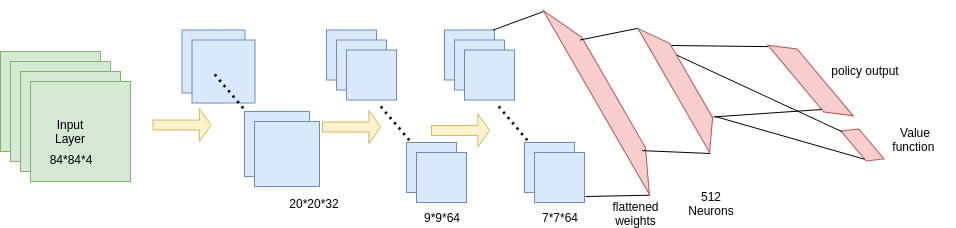
\includegraphics[scale=0.5]{Network}\\

The first layer is the input, which consists of the raw visual feed of the game, and 4 such frames are stacked on each other. \\
The next one is a concolutional layer with kernel size=8 and the stride of 4, which reduces the dimension of the image to 20*20. There are 32 such filters. \\
The next convolutional layer reduces the filter size to 9*9, there are 64 such channels, the next layer reduces the size to 7*7 with the same number of channels. \\
The last convolutinal layer is flattened to obtain 7*7*64=3136 neurons. This layer is fullly connected to 512 neurons in the next layer. \\
The 512-neuron layer is then connected to separate outputs corresponding the policy and the value outputs. \\


\section{Training Loop}
And finally we initialise the Model() of out Neural network. 
The model consists of 3 convolutional layers, and two fully connected layer. 
The models predicts the Policy($\pi$) and the Values function of the state. 

\begin{lstlisting}
	def run_training_loop(self):

		loss_vec=[]
		rewards_vec=[]

		episode_info=deque(maxlen=100)
		for update in range(self.updates):
			time_start=time.time()
			progress =update/self.updates

			learning_rate=3e-4 *(1-progress)
			clip_range= 0.1*(1-progress)

			samples, samples_episode_info=self.sample()
			
			info_loss=self.train(samples, learning_rate, clip_range)
			
			time_end=time.time()

			fps=int(self.batch_size/(time_end-time_start))

			episode_info.extend(samples_episode_info)
			
			reward_mean, length_mean =Main._get_mean_episode_info(episode_info)
			sampled_rewards= samples['rewards'].data.numpy()
			rew_total=sampled_rewards.sum()

			loss_err=info_loss[5].data.numpy()
			rew_np=reward_mean#reward_mean.data.numpy()

			print loss_err, 'training loss \n'
			loss_vec.append(loss_err)
			rewards_vec.append(rew_total)

			print("f",update,": fps=",{fps} ,'reward',{rew_total},' length',{length_mean}, info_loss)
			if update%10==0 and update!=0:

				np.save('loss_vec1_breakout', loss_vec)
				np.save('reward_vec1_breakout', rewards_vec)


\end{lstlisting}

After having initialized the model, we now begin the training process. \\
self.updates represents the number of times the sampling procedure, and optimization is going to take place. \\
Learning rate, is initialized as a function of the progress percentage, this is used to anneal the learning rate. clip range is also varied similarly. \\
\newline
samples is the vector containing the information stored from the function self.sample(). 
\subsection{def sample():}

This function is used to sample trajectories from the current policy.
\begin{lstlisting}
	def sample(self):
		
		rewards=np.zeros((self.n_workers, self.worker_steps), dtype=np.float32)
		actions=np.zeros((self.n_workers, self.worker_steps), dtype=np.int32)
		dones = np.zeros((self.n_workers, self.worker_steps), dtype=np.bool)
		obs = np.zeros((self.n_workers, self.worker_steps, 84, 84, 4), dtype=np.uint8)
		neg_log_pis = np.zeros((self.n_workers, self.worker_steps), dtype=np.float32)
		values = np.zeros((self.n_workers, self.worker_steps), dtype=np.float32)
		episode_infos = []

		for t in range(self.worker_steps):
			obs[:,t]=self.obs
			pi,v=self.model(obs_to_torch(self.obs))

			values[:, t] = v.cpu().data.numpy()
			
			a=pi.sample()
			actions[:,t]=a.cpu().data.numpy()
			
			neg_log_pis[:,t]=-pi.log_prob(a).cpu().data.numpy()

			for w,worker in enumerate(self.workers):

				worker.child.send(("step",actions[w,t]))

			for w, worker in enumerate(self.workers):
				
				self.obs[w], rewards[w,t], dones[w,t], info=worker.child.recv()


				if info:
					info['obs']=obs[w,t,:,:,3]
					episode_infos.append(info)

		advantages = self._calc_advantages(dones, rewards, values)

		samples={'obs':obs, 'actions':actions, 'values':values, 'neg_log_pis':neg_log_pis, 'advantages':advantages, 'rewards':rewards}

		samples_flat={}
		for k,v in samples.items():
			v=v.reshape(v.shape[0]*v.shape[1], *v.shape[2:])

			if k=='obs':
				samples_flat[k]=obs_to_torch(v)
			else:
				samples_flat[k]= torch.tensor(v, device=device)
		return samples_flat, episode_infos
\end{lstlisting}



The first part of the sampling process is initializing the tensors for rewards, actions, dones, observations, value functions, and negative log likelihood. \\
np.zeros is used to initialize the tensors for each of these entities.

Now for a range of worker steps,all of the information will be filled by taking sequential steps, for each worker and filling in the information relevant to each step

\subsection{Calculating the Advantage}

\begin{lstlisting}
	def _calc_advantages(self, dones, rewards, values):

		advantages=np.zeros((self.n_workers, self.worker_steps), dtype=np.float32)
		last_advantage=0

		_,last_value= self.model(obs_to_torch(self.obs))
		last_value= last_value.cpu().data.numpy()

		for t in reversed(range(self.worker_steps)):
			mask=1.0-dones[:,t]
			last_value =last_value*mask
			last_advantage=last_advantage*mask

			delta =rewards[:,t]+self.gamma*last_value -values[:,t]
			last_advantage=delta+self.gamma*self.lamda*last_advantage

			advantages[:,t]=last_advantage
			last_value=values[:,t]

		return advantages
\end{lstlisting}

\subsubsection{Maths}
$\hat{A_t^{1}}$=$r_t+\gamma V(s_{t+1})-V(s)$\\
$\hat{A_t^{2}}$=$r_t+\gamma r_{t+1}+\gamma^2 V(s_{t+2})-V(s)$\\
...\\
$\hat{A_t^{\infty}}$=$r_t+\gamma r_{t+1}+\gamma^2 r_{t+2}+...-V(s)$\\

The first advantage function $\hat{A_t^{1}}$ has a high bias, and low variance, whereas $\hat{A_t^{\infty}}$ has high variance but low bias. We want a tradeoff between these advantage functions, hence we take a weighted sum of all the advantages, called Generalized advantage estimation, $\hat{A_t^{GAE}}=\Sigma_k w_k \hat{A_t^{k}} $\\

$w_k$ is set as $\lambda^{k-1}$\\
$\hat{A_t^{GAE}}=\frac{1}{1-\lambda}[\hat{A_t^{1}} + \lambda \hat{A_t^{2}}+...+\lambda^{k-1} \hat{A_t^{\infty}}] $\\
\newline
We use $\delta_t$ which is much easier to deal with that calculating advantage functions. \\

$\delta_t=r_t+\gamma V(s_{t+1})-V(s_t)$


$\hat{A_t} = \delta_t+ \gamma \lambda \delta_{t+1}+ ....+ (\gamma \lambda)^{T-t+1}\delta_{T-1} =\delta_t+ \gamma \lambda \hat{A_{t+1}}$\\
\newline
Usign these equations, we can calculate the advantage function recursively for all the states encountered. Key thing to notice is that we are reversing the order of the states, ie we start by calculating advantage for the last state fisrt and then move to the last second. \\
\newline
Now we are done calculating all the relevant information of the samples. 
\newline
The next part of the process is training

\subsection{Train}
This is the part where we are training the model using the generated samples from out current policy. We plan to improve our current policy. 

\begin{lstlisting}
	def train(self, samples, learning_rate, clip_range):

		train_info=[]

		for _ in range(self.epochs):

			indexes=torch.randperm(self.batch_size)

			for start in range(0, self.batch_size, self.mini_batch_size):

				end=start+self.mini_batch_size
				mini_batch_indexes =indexes[start:end]
				mini_batch={}

				for k,v in samples.items():
					mini_batch[k]=v[mini_batch_indexes]

				res=self.trainer.train(learning_rate=learning_rate, 		    clip_range=clip_range, samples=mini_batch)

				train_info.append(res)
		return np.mean(train_info, axis=0)
\end{lstlisting}

We are taking input as the samples(consisting of obs,actions,values,advantages,and rewards).\\
Now we divide the current data into certain minibatches, 
and then train model, using these minibatches. \\
\newline 
Trainer.train fuction will be used to finally train using the mini-batches. 

\section{Class Trainer}
First of all, the mode of optimization is set. We are going to use torch.optim.Adam for the optimizatin process. \\
\newline
Trainer.train takes in the samples, which is the mini-batch in this case and also the learning rate and the clip range. We will discuss what is clip range in details. \\
First part is creating local variables for all the attributes of the samples. \\

The current policy is generated, for all the samples in the dataset. this is stored in pi, value. \\
Next, we will look at the derivation for the loss function. \\
\subsection{Maths}
The content for this part is borrowed from \textbf{Berkeley Deep RL course} and \textbf{PPO paper}. 
\newline
Policy Gradient methods try to optimize the function 
\begin{center}
$max_{\theta} J(\pi_{\theta})=E_{\tau=\pi_{\theta}}[\Sigma_{t=0}^{\infty}\gamma^{t} r_t]$
\end{center}
The equation is optimized for $\theta$, but the sample efficiency is poor. the data is thrown out after one update, and distance in parameter space does not correspond to distance in policy space. \\
PPO used the concept of relative policy performance, to update the parameters. 
ie.
\begin{center}
$max_{\pi^{new}}J(\pi^{new})=max_{\pi^{new}}J(\pi^{new})- J(\pi^{old})$
\end{center}
Here, $\pi^{new}$ represents the new policy, and $\pi^{old}$ is the old policy. \\
\newline
We need to find a more simplified version of the above expression. \\

\begin{equation}
\begin{aligned}
J(\pi^{new})- J(\pi^{old}) &= J(\pi^{new})-E_{\tau \sim \pi^{new}}[V^{\pi_{old}}(s_0)] \\
& = J(\pi^{new})+ E_{\tau \sim \pi^{new}}[\Sigma_{t=1}^{\infty} \gamma^t V^{\pi_{old}}(s_t)-\Sigma_{t=0}^{\infty} \gamma^t V^{\pi_{old}}(s_t)]\\
& = J(\pi^{new})+ E_{\tau \sim \pi^{new}}[\Sigma_{t=0}^{\infty} \gamma^{t+1} V^{\pi_{old}}(s_{t+1})-\Sigma_{t=0}^{\infty} \gamma^t V^{\pi_{old}}(s_t)]\\
& =E_{\tau \sim \pi^{new}}[\Sigma_{t=0}^{\infty}\gamma^t(R(s_t,a_t,s_{t+1})) +\gamma V^{\pi_{old}}(s_{t+1})-V^{\pi_{old}}(s_t)]\\
& = E_{\tau \sim \pi^{new}}[\Sigma_{t=0}^{\infty} \gamma^t A^{\pi}(s_t,a_t)]\\
& = \frac{1}{1-\gamma} E_{s \sim d^{\pi_{new}}, a \sim \pi^{new}} [A^{\pi}(s_t,a_t)]\\
& = \frac{1}{1-\gamma} E_{s \sim d^{\pi_{new}}, a \sim \pi^{old}} [ \frac{\pi^{new}(a|s)}{\pi^{old}(a|s)}A^{\pi}(s_t,a_t)] (importance-sampling)\\
\end{aligned}
\end{equation}
The only problem with the given equation is that we cannot sample from $d^{\pi_{new}}$, so we say that $d^{\pi_{new}}=d^{\pi_{old}}$ and this assumption turns out to be pretty good, becuase there is not much difference in the discounted state distribution. 
\newline
We denote this as $L^{CPI}(\theta)$.
Without constraint, $L^{CPI}(\theta)$ would lead to excessively large policy updates. Therefore, large policy updates are constrained.\\
 $r_t(\theta)=\frac{\pi^{new}(a|s)}{\pi^{old}(a|s)}A^{\pi}(s_t,a_t)$\\
\begin{center}$L^{CLIP}(\theta)=\hat{E}_t[min(r_t(\theta), clip(r_t(\theta), 1-\epsilon, 1+\epsilon)\hat{A}_t)]$\\
\end{center}

This is the main proposed objective function. 
\subsection{code}
\begin{lstlisting}
class Trainer:
	def __init__(self, model):
		self.model=model
		#print(self.model.parameters())
		self.optimizer=torch.optim.Adam(self.model.parameters(),lr=3e-4)

	def train(self, samples,  learning_rate, clip_range):
		sampled_obs= samples['obs']
		sampled_action= samples['actions']
		sampled_return= samples['values'] +samples['advantages']
		sampled_normalized_advantage=Trainer._normalize(samples['advantages'])
		sampled_neg_log_pi=samples['neg_log_pis']
		sampled_value=samples['values']

		pi,value= self.model(sampled_obs)

		neg_log_pi=-pi.log_prob(sampled_action)
		ratio=torch.exp(sampled_neg_log_pi-neg_log_pi)

		clipped_ratio=ratio.clamp(min=1.0-clip_range, max=1.0+clip_range)
		policy_reward=torch.min(ratio*sampled_normalized_advantage,clipped_ratio*sampled_normalized_advantage)
		policy_reward=policy_reward.mean()
		entropy_bonus=pi.entropy()
		entropy_bonus=entropy_bonus.mean()

		clipped_value= sampled_value+(value-sampled_value).clamp(min=-clip_range, max=clip_range)
		vf_loss=torch.max((value-sampled_return)**2, (clipped_value-sampled_return)**2)
		vf_loss=0.5* vf_loss.mean()
		loss=-(policy_reward-0.5*vf_loss+0.01*entropy_bonus) #policy_reward#

		for pg in self.optimizer.param_groups:
			pg['lr']=learning_rate
		self.optimizer.zero_grad()
		loss.backward()
		torch.nn.utils.clip_grad_norm_(self.model.parameters(),max_norm=0.5)
		self.optimizer.step()

		approx_kl_divergence = .5 * ((neg_log_pi - sampled_neg_log_pi) ** 2).mean()
		clip_fraction=(abs((ratio-1.0))>clip_range).type(torch.FloatTensor).mean()
		return [policy_reward, vf_loss, entropy_bonus, approx_kl_divergence, clip_fraction, loss]

	@staticmethod
	def _normalize(adv):
		return (adv-adv.mean())/(adv.std()+1e-8)

\end{lstlisting}
 

\section{Record Video}

Once the model has traied fairly well, we can use the function record-video to record the video of the game being played by the agent. \\
It does the job of sampling trajectories for multiple workers, and then, it stores the images in a particular specified folder with a certain pattern. \\

\begin{lstlisting}
	def record_video(self):

		samples, samples_episode_info=self.sample_video()
		print np.shape(samples["obs"])
		n_worker=np.shape(samples["obs"][0])
		n_episodes=	np.shape(samples["obs"][1])
		obs=samples["obs"]
		for worker in range(8):		
			for frame in range(128):

				img=obs[worker,frame,:,:,1]	
				frame_str=str(frame).zfill(4)
				name='image'+str(worker)+'k'+frame_str+'.png' #/home/abhijeet/Desktop/Practise_code/RL
				print name
				cv2.imwrite('img_break/'+name, img)
\end{lstlisting}

We can use the command avconv to combine these images to create a video. 
have a look at the avconv documentation for more details. 
\begin{lstlisting}
avconv -f image2 -i image1b%d.png -r 76 -s 800x600 video1.avi
\end{lstlisting}
\end{document}
